%%%%%%%%%%%%%%%%%%%%%%%%%%%%%%%%%%%%%%%%%%%%%%%%%%%%%%%%%%%%%%%%%%%%%%%%%%%%%%%%
%2345678901234567890123456789012345678901234567890123456789012345678901234567890
%        1         2         3         4         5         6         7         8

\documentclass[letterpaper, 10 pt, conference]{ieeeconf}  % Comment this line out if you need a4paper

%\documentclass[a4paper, 10pt, conference]{ieeeconf}      % Use this line for a4 paper

\IEEEoverridecommandlockouts                              % This command is only needed if 
                                                          % you want to use the \thanks command

\overrideIEEEmargins                                      % Needed to meet printer requirements.

% See the \addtolength command later in the file to balance the column lengths
% on the last page of the document

% The following packages can be found on http:\\www.ctan.org
\usepackage{graphics} % for pdf, bitmapped graphics files
\usepackage{epsfig} % for postscript graphics files
%\usepackage{mathptmx} % assumes new font selection scheme installed
%\usepackage{times} % assumes new font selection scheme installed
\usepackage{amsmath} % assumes amsmath package installed
%\usepackage{amssymb}  % assumes amsmath package installed
\usepackage{amsfonts}
\usepackage{bm}
\usepackage{cite}

\title{\LARGE \bf
Wind Disturbance Rejection for Unmanned Aerial Vehicle Based on Estimated Acceleration Feedback*
}

\author{Bo Dai$^{1,2}$, Yuqing He$^{2}$, Guangyu Zhang$^{1,2}$, Feng Gu$^{2}$, Liying Yang$^{2}$, Jianda Han$^{2}$, and Weiliang Xu$^{3}$% <-this % stops a space
\thanks{*This work is supported by the National Natural Foundation of China (Grant No. 61433016 and 61503369) and the State Key Laboratory of Robotics, Shenyang Institute of Automation, China.}% <-this % stops a space
\thanks{$^{1}$University of Chinese Academy of Sciences, Beijing 100049, China.
    {\tt\small \{daibo,zhangguangyu\}@sia.cn}}%
\thanks{$^{2}$The State Key Laboratory of Robotics, Shenyang Institute of Automation, Chinese Academy of Sciences, Shenyang 110016, China.
    {\tt\small \{heyuqing,fenggu,yangliying,jdhan\}@sia.cn}}%
\thanks{$^{3}$Weilinag Xu is with Department of Mechanical Engineering, the University of Auckland, Auckland, New Zealand.
    {\tt\small p.xu@auckland.ac.nz}}
}


\begin{document}

\maketitle
\thispagestyle{empty}
\pagestyle{empty}


%%%%%%%%%%%%%%%%%%%%%%%%%%%%%%%%%%%%%%%%%%%%%%%%%%%%%%%%%%%%%%%%%%%%%%%%%%%%%%%%
\begin{abstract}

Wind disturbance has been a critical issue for safety flight of unmanned aerial vehicle (UAV) and increases the challenges for control system design.
To this end, an acceleration feedback enhanced method is applied for wind disturbance rejection of UAV.
In this paper, a modified acceleration, including linear and angular acceleration, feedback method with a pre-filter is designed and tested on a hex-rotor.
In order to make it easy to add acceleration feedback method into a model free control structure such as cascaded PID controller used in the hex-rotor, a novel, effective and simple method for parameters identification of multi-rotor is proposed, along with an online acceleration estimator based on \textsl{Kalman Filter}.
Finally, two types of wind, continuous and gusty wind, are analyzed and taken into consideration in the experiment.
The comparison results of hovering performance between PID controller and acceleration feedback enhanced PID controller verify that the proposed method is not robust but effective for both types of wind disturbances.

\end{abstract}

%%%%%%%%%%%%%%%%%%%%%%%%%%%%%%%%%%%%%%%%%%%%%%%%%%%%%%%%%%%%%%%%%%%%%%%%%%%%%%%%
\section{Introduction}

UAV has drawn increasing attention from robotics community over the last decades, and it has been used wildly in military and civilian applications such as border patrol \cite{Girard2004}, search and rescue \cite{Qi2016}, surveillance and aerial photography.
However, the operation environments of UAV always exist various threats such as the vehicle downwash when operating close to walls and floors, turbulent airflow when flight between buildings \cite{Waslander2009} and strong wind during adverse weather.
In fact, wind disturbance is the most general and primary type of disturbance to UAV since that almost all power of it comes from the relative motion with air.
Strong wind disturbance may cause losing control of the UAV and even lead to crash, or may weaken stability and downgrade performance of the system such as positioning accuracy reduction and attitude swaying, which may not threaten the safety of UAV but can cause the failure of missions.
Thus, robustness against wind disturbance is one of the critical issue, which must be considered in control system design to obtain high performance of UAV.

So far, numerous remarkable work has been focusing on disturbance rejection control to improve the robustness of the UAV.
Among all these work, methods for disturbance rejection can be mainly divided into two types.
The first one is that controller is designed based on the dynamic model of the system and it can suppress the disturbance itself such as proportional integral derivative (PID) based controller, $H_{\infty}$ \cite{He2007} and some nonlinear methods such as nested saturation control \cite{Nicotra2014} and backstepping \cite{Madani2006}.
PID controller is the most classical and wildly used since its simple structure, clear parameters and easy implementation. But parameters turning of PID needs lots of experiments and rich experiences to obtain high precision control performance.
$H_{\infty}$ control is well known robust against uncertainties and modeling errors and yet it is difficult to achieve a balance between robustness and conservation since the uncertainty is usually supposed unknown \cite{He2010}.
Nested saturation control and backstepping are examples of nonlinear control techniques able to provide larger regions of attraction.
The second type of disturbance rejection method is based on known disturbance or the states those contain disturbance information, which can be called disturbance based control (DBC).
The key of it is the accurate estimation of disturbance or obtaining the relationship between disturbances and system states.
There are two distinct approaches for disturbance observer including time-domain disturbance observer (DOB) and frequency-domain DOB \cite{Su2016}.
Extended state observer (ESO) is one of the time-domain DOB.
It expands the disturbances and uncertainties as system states, then a state observer is designed to estimate these states.
ESO also plays a vital part in active disturbance rejection control (ADRC) method \cite{Han2009}.
The original frequency-domain DOB is proposed by Ohishi et al.\cite{Ohishi1987}, and the key of it is obtaining disturbance estimation by filtering the differences between control input and the calculated input using the inverse mode of nominal plant.
Recently, it has been starting deploying on multi-rotor for real time disturbance rejection control \cite{Tomic2014}.

Whether external disturbances of force and torque or internal disturbance of parameter perturbation, the effects of them are always reflected by acceleration information (including linear and angular acceleration).
Thus, acceleration based method has been researched and applied for disturbance rejection, and it also belongs to DBC method.
Acceleration feedback (AF) control method is first proposed and applied by Studenny and Belanger in \cite{Studenny1984}. In our previous work \cite{Xu2000,Han2000}, the applications of AF method on force control and direct-driver manipulator control demonstrates this method is not feasible but effective for robot control.
Moreover, AF enhanced robust control combined with $H_{\infty}$ method has been applied on unmanned helicopter control, and the simulation results demonstrate the improvements of the method \cite{He2007,He2010}.

In this paper, an AF enhanced controller, proposed in our previous work \cite{He2010}, is designed for UAV control and the encouraging experimental results verify the reliability and effectiveness of the method for wind disturbance rejection.
In fact, there are many remarkable efforts focusing on wind disturbance problem for UAV as can be found in \cite{Tomic2014,Escareno2013,Lee2016,Cabecinhas2015,Leonard2012}. But some of them present only simulation results or are tested on tested without real flight.
They all lack the analysis of wind fields, and the wind may not strong enough to effect UAV.
Thus, the main contributions of this paper are threefold:

\begin{itemize}
    \item It is the first time that applying AF method on practical UAV system for wind disturbance rejection control and achieving significant success.
    \item The effects on the vehicle of wind disturbance with particular frequency are analyzed, which provides the reference for AF enhanced controller design.
    \item A novel, effective and simple method for parameters identification of UAV is proposed, which sets up a bridge from none model control to model based control and provides the basis for AF method.
\end{itemize}

The remainder of this paper is organized as follows. The theoretical analysis of AF method is introduced in Section II along with a modified AF method proposed in our previous work \cite{He2010}.
Section III introduces the model of a hex-rotor used for experiment as well the designed AF controller for it.
Then experimental implementation will be detailed in Section IV including an online acceleration estimator based on \textsl{Kalman Filter} and a novel method for parameters identification of UAV.
And the analyses of experimental results are presented in Section V.
Finally, some concluding remarks are drawn in Section VI.

\section{Acceleration Feedback Enhanced Method}

\subsection{High Gain AF Method}

The general dynamic model of a mechatronic system with multiple freedom, which includes UAV system, is established by Euler-Lagrange equation as
\begin{equation}
    M(q)\ddot{q}+C(q,\dot{q})\dot{q}+G(q)+F(q,\dot{q})=\tau+\Delta 
    \label{e1} 
\end{equation}
where $q\in\mathbb{R}^n$ is position vector, and $M(q)$ is mass as a scale.
$C(q,\dot{q})\in\mathbb{R}^n$, $G(q)\in\mathbb{R}^n$ and $F(q,\dot{q})\in\mathbb{R}^n$ are Coriolis force, gravity and drag force respectively.
However, this equation also holds when $q$ represents angular displacements, and the meaning of other valuables would change as well, such as $M(q)$ would be the inertial tensor matrix and belongs to $\mathbb{R}^n\times\mathbb{R}^n$, where $\tau$ and $\Delta$ would be driving torque and disturbance torque respectively.
High gain AF is an enhanced control method suitable for single input single output system, and it has been verified in many mechatronic systems \cite{Studenny1984,Xu2000,Han2000}. Here, we consider any freedom in (\ref{e1})
\begin{equation}
    J_{ii}\ddot{q}_i = \tau_i + \tau_{ui}
    \label{e2}
\end{equation}
where $J_{ii}$ is an inertial coefficient which could be mass or moment of inertia, and
\begin{equation}
    \tau_{ui}=\Delta_i - \sum_{j=1}^{n}C_{ij}(q,\dot{q})\dot{q}_j - G_{ii}(q) - F_{ii}(q,\dot{q}) 
    \label{e3}
\end{equation}
consists of various coupling force (torque) and external disturbance force (torque), which is also called uncertainty.

The key point of high gain AF is turning (\ref{e2}) from force (torque) driving to acceleration (linear or angular acceleration) driving, so that the disturbance can be suppressed. The controller of high gain AF is determined by
\begin{equation}
    \tau_i=k_a(v-\ddot{q}_i) \label{e4}
\end{equation}
where $k_a$ is a positive constant and called the gain of acceleration feedback.
Combining (\ref{e2}) and (\ref{e4}), we can obtain
\begin{equation}
    \ddot{q}_i=\frac{k_a}{J_{ii}+k_a} v + \frac{1}{J_{ii}+k_a}\tau_{ui} 
    \label{e5}
\end{equation}
if $k_a$ is chosen big enough, that is $k_a\gg 1$, $k_a\gg J_{ii}$, then
\begin{equation}
    \ddot{q}_i\approx v 
    \label{e6}
\end{equation}
Thus, we obtain a new acceleration tracking controller which can track the reference input.
Moreover, the uncertainty $\tau_{ui}$ is suppressed in a large extent.
But it may exist two problems when applied it on practical system.

The first problem is algebraic loop.
Substitute (\ref{e4}) into (\ref{e2}), then
\begin{equation}
    J_{ii}\ddot{q}_i=k_a(v-\ddot{q}_i) + \tau_{ui}
    \label{e7}
\end{equation}
where exists two acceleration parts.
To present more clearly, Fig. \ref{f1} gives an illustration of (\ref{e7}), where the thick lines represent acceleration feedback loop.
Apparently, in this loop, there is no dynamic link, which occurs an algebraic loop.
However, algebraic loop is not allowed in practical system since it will increase the instability and weaken the transient response of the system.
The second one is the implementation of high gain.
As we mention above, the key to suppress disturbance is the high gain of AF $k_a$.
However, in many cases, this is difficult or even forbidden in practical system due to the flexible limitation and unmodeled dynamics of the system.
If the implementation of high gain is invalid, the cornerstone of high gain AF would collapse.
Although some work improves this shortcoming such as \cite{Han2000}, it increases the complexity of control design and reduces the generality of this method.
% The last problem is AF cannot deal with nonlinear system, because the all nonlinearities are taken as disturbance and suppressed in high gain AF method.
% While in many practical system, some nonlinearities or can be modeled accurately, and if it is put to good use, the performance of closed loop of the system will be improved greatly.
\begin{figure}[t]
    \centering
    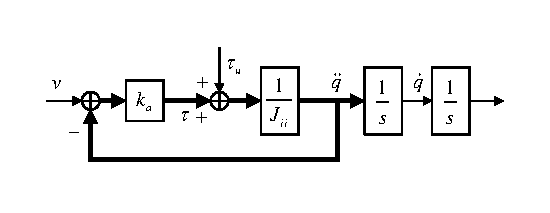
\includegraphics[width=2.95in]{illustrations/fig1.pdf}
    \caption{Sketch of algebraic loop in high-gain AF}
    \label{f1}
\end{figure}

\subsection{Modified AF Method with a Pre-filter}
In order to overcome the problems mentioned above, a modified AF method with a pre-filter is proposed.
Combining (\ref{e2}) and (\ref{e4}), then
\begin{equation}
    \tau_{i} = \frac{k_a}{1+ k_a / J_{ii}} - \frac{k_a}{J_{ii}+k_a} \tau_{ui}
    \label{e8}
\end{equation}
A new sketch of (\ref{e8}) is illustrated in Fig. \ref{f2}, and it is equivalent to Fig. \ref{f1}
Thus, we can conclude that the essence of high gain AF is that disturbance rejection is based on known disturbance information.
The measured acceleration can be utilized to calculate the disturbance information, but it also contains control input $\tau_i$.
It will appear that the input of current moment is determined by current measurement, which directly causes algebraic loop.
Thus, the key to eliminate algebraic loop is avoiding the static process from acceleration measurement to control input.
\begin{figure}[t]
    \centering
    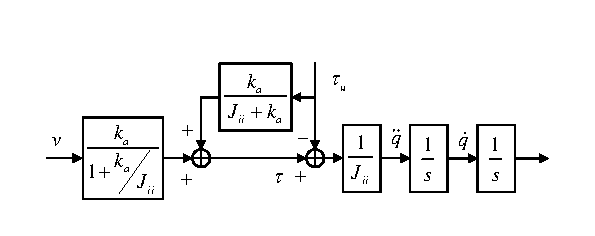
\includegraphics[width=2.95in]{illustrations/fig2.pdf}
    \caption{A new sketch of high gain AF}
    \label{f2}
\end{figure}

Based on the analysis above, we utilize acceleration information to obtain disturbance rather than adding an acceleration close loop directly, then to avoid algebraic loop, a dynamic process, also called pre-filter, is added into controller which turns (\ref{e8}) into
\begin{equation}
    \tau_i=\frac{k_a}{1+k_a / J_{ii}}v - \frac{k_a}{J_{ii}+k_a}\frac{B(s)}{A(s)}\tau_{ui}
    \label{e9}
\end{equation}
Substitute (\ref{e9}) into (\ref{e2}), then any freedom of the system can be described as
\begin{equation}
    J_{ii}\ddot{q}_i = \frac{1/k_a}{1/J_{ii}}v - \frac{B(s)-(J_{ii}/k_a+1)A(s)}{(J_{ii}/k_a+1)A(s)}\tau_{ui}
    \label{e10}
\end{equation}

The sketch of the new AF is shown in Fig. \ref{f3}.
The algebraic loop is eliminated by adding a pre-filter, but it increases the difficulty of controller design as well.
Fortunately, the gain of AF $k_a$ in the controller is only in the form of reciprocal in (\ref{e10}), and a bigger $k_a$ results in stronger a disturbance rejection effect.
Thus, let $k_a\rightarrow\infty$, that is $k_a\gg max(1,J_{ii})$, then (\ref{e9}) and (\ref{e10}) are approximated as
\begin{equation}
    \tau_i = J_{ii}v - \frac{B(s)}{A(s)}\tau_{ui} 
    \label{e11}
\end{equation}
\begin{equation}
    J_{ii}\ddot{q}_i = J_{ii}v + \frac{A(s) - B(s)}{A(s)}\tau_{ui} 
    \label{e12}
\end{equation}
\begin{figure}[t]
    \centering
    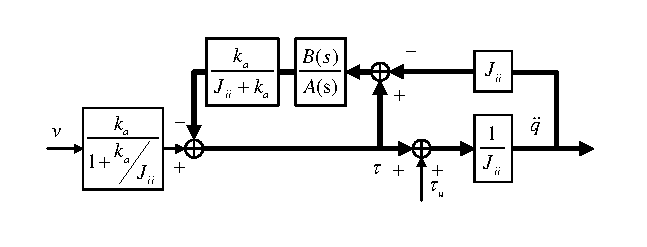
\includegraphics[width=2.95in]{illustrations/fig3.pdf}
    \caption{Modification by adding a pre-filter}
    \label{f3}
\end{figure}

The new controller is shown in Fig. \ref{f4}
As can be seen, the gain of AF $k_a$ is no more than a process value witch only exists in analysis and disappears in controller structure.
Although gain $k_a$ is chosen to be infinity, it does not cause any problem in implementation.
Thus, the key to suppress disturbance is not the gain $k_a$ anymore but the dynamic process determined by $A(s)$ and $B(s)$.

\begin{figure}[h]
    \centering
    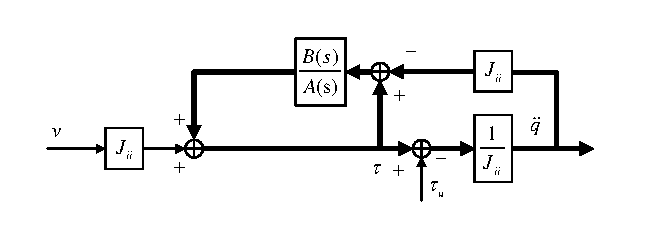
\includegraphics[width=2.95in]{illustrations/fig4.pdf}
    \caption{Sketch of pre-filter based AF}
    \label{f4}
\end{figure}

Actually, as can be seen in (\ref{e12}), uncertainty $\tau_{ui}$ effects system after filtered by
\begin{equation}
    Q(s) = \frac{A(s)-B(s)}{A(s)} 
    \label{e13}
\end{equation}
Thus, we can determine a proper $Q(s)$ based on main frequency of uncertainty $\tau_{ui}$.
Normally, the uncertainty or disturbance of the system is at low frequency level.
A high pass filter will be ale to suppress the disturbance, for example, if we chose
\begin{equation}
    \frac{B(s)}{A(s)} = \frac{a}{s+a}, Q(s) = \frac{s}{s+a} \label{e14}
\end{equation}
then
\begin{equation}
    J_{ii}\ddot{q}_i = J_{ii}v + \frac{s}{s+a}\tau_{ui} \label{e15}
\end{equation}
Thus, the disturbance with low frequency in $\tau_{ui}$ would be filtered, and the cut frequency of this high pass filter is determined by $a$.

\section{System Model and Controller Design}

\subsection{System Model}

A hex-rotor is used as an UAV platform to verify our method.
It is a kind of multi-rotor and has six identical rotors and propellers located at the vertices of a regular hexagon as shown in Fig. \ref{f5}.
Hex-rotor is modeled as a rigid body with multiple freedom, and of cause, it is a special case of mechatronic system mentioned in Section II.
\begin{figure}[t]
    \centering
    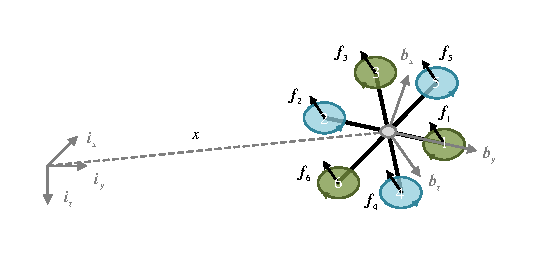
\includegraphics[width=2.95in]{illustrations/fig5.pdf}
    \caption{Illustration of hex-rotor}
    \label{f5}
\end{figure}

Two frames, an inertial reference frame $\{\bm{i_x},\bm{i_y},\bm{i_z}\}$ and a body-fixed frame $\{\bm{b_x},\bm{b_y},\bm{b_z}\}$, are involved.
And the origin of the body-fixed frame is located at the center of the mass.
The first and the second axis of body-fexed frame, $\bm{b_x}$ and $\bm{b_y}$, lie along the symmetry axes of the vehicle as shown in Fig. \ref{f5}, and the third axis $\bm{b_z}$ is normal to $\bm{b_x}$ and $\bm{b_y}$ and points downward.
The configuration of this hex-rotor UAV is defined by location of the center of mass and the attitude with respect to the inertial frame.
Thus, the configuration manifold is the special Euclidean group $\mathfrak{se}(3)$ and special orthogonal group $\mathfrak{so}(3)=\{R\in \mathbb{R}^{3\times 3} |R^TR=I, det R=1\}$, and $R$ is the rotation matrix from body-fixed frame to inertial frame.

We suppose that the thrust of each propeller is normal to the quadrotor plane, and the thrust of each propeller $f_i$ can be approximaed by
\begin{equation}
    f_i = \kappa\Omega^2_i \label{e16}
\end{equation}
where $\Omega_i$ is the rotation speed of each rotor. 
Then, the total thrust of the propellers is $f=\sum_{i=1}^6f_i$ along the direction of $\bm{-b_z}$.
Therefore, the total thrust can be given by $-fR\bm{e_3}\in\mathbb{R}^3$ in the inertial frame, where $\bm{e}_3 = [0,0,1]^T$.
We also assume the torque generated by each propeller is directly proportional to its thrust.
Given that there are three propellers rotate clockwise and the others rotate counterclockwise as shown in Fig. 5, thus the torque generated by each propeller is $\tau_i=\pm c_{\tau f}f_i$, for a fixed constant $c_{\tau f}$.
Under these assumptions, and the special structure of hex-rotor, the total thrust $f$ and the total moment $M$ generated by propellers can be written as
\begin{equation}
    \begin{bmatrix}
        f \\ M_1 \\ M_2 \\ M_3 \\
    \end{bmatrix} = 
    \begin{bmatrix}
        1 & 1 & 1 & 1 & 1 & 1 \\
        -d & d & \frac 12 d & -\frac 12 d & -\frac 12 d & \frac 12 d \\
        0 & 0 & \frac{\sqrt3}{2} d & -\frac{\sqrt3}{2} & \frac{\sqrt3}{2} & -\frac{\sqrt3}{2} \\
        -c_{\tau f} & c_{\tau f} & -c_{\tau f} & c_{\tau f} & c_{\tau f} & -c_{\tau f}
    \end{bmatrix}
    \begin{bmatrix}
        f_1 \\ f_2 \\ f_3 \\ f_4 \\ f_5 \\ f_6
    \end{bmatrix}
    \label{e17}
\end{equation}
where $d$ is the distance from propeller center to the origin of body-fixed frame.
For a given $f$ and $M$, the thrust of each rotor $f_i$ can be obtained by calculating the generalized inverse of (\ref{e17}).
The motion of the UAV can be described as
\begin{equation}
    \left\{
        \begin{aligned}
            & m\ddot{x}=mg\bm{e}_3-fR\bm{e}_3+d_f \\
            & J\dot{\omega}=M-\omega\times J\omega + d_\tau
        \end{aligned}
    \right.
    \label{e18}
\end{equation}
where $m$, $g$ and $d_f$ are the total mass, acceleration of gravity and disturbance force or uncertainty respectively, and $J$, $\omega$ and $d_\tau$ are the moment of inertia, angular velocity and disturbance torque respectively.

\subsection{Controller Design}

Consider linear motion of hex-rotor in (\ref{e18}) without any disturbance under ideal situation
\begin{equation}
    m\ddot{x}_d = F_d - mg\bm{e}_3
    \label{e19}
\end{equation}
where $\ddot{x}_d$ is desired acceleration and $F_d$ is desired force. However, there exists a disturbance $d_f$ in practical system along with a desired AF enhanced term $v_f$
\begin{equation}
    m\ddot{x} = F_d - mg\bm{e}_3 + v_f + d_f
    \label{e20}
\end{equation}
where $\ddot{x}$ is the real acceleration measured by online sensor.
As described in Section II, $v_f$ and $d_f$ should satisfy
\begin{equation}
    \frac{v_f(s)+d_f(s)}{d_f(s)} = Q(s)
    \label{e21}
\end{equation}
If $A(s)$ and $B(s)$ are chosen as (\ref{e14}), combine it with (\ref{e19}) and (\ref{e20}), the designed AF enhanced term is decided by
\begin{equation}
    v_f(t) = a\int (F_d - mg\bm{e}_3 + m\ddot{x})dt 
    \label{e22}
\end{equation}

The design of AF method on angular motion is as same as the process above, and the AF enhanced term should be
\begin{equation}
    v_\tau(t) = b\int (M_d - \omega\times J\omega + J\ddot{q})dt
    \label{e23}
\end{equation}
where $b$ is the cut frequency as described in (\ref{e15}), $M_d$ is the designed torque generated by a stable controller, and $\ddot{q}$ is angular acceleration measured by sensor.

As can be seen above, the design of AF enhanced term is independent with the design of the controller.
The control structure of the hex-rotor in our experiment is illustrated in Fig. \ref{f6}.
The control input is desired position $x_d$ and yaw $\psi_d$.
In position and velocity controller, a cascade PID is used to generate desired force $F_d$ and z-axis of body-fix frame $\bm{b}_{zd}$.
Then in attitude controller, geometric tracking control \cite{Lee2010} is used to generate desired torque $M_d$.
\begin{figure}[t]
    \centering
    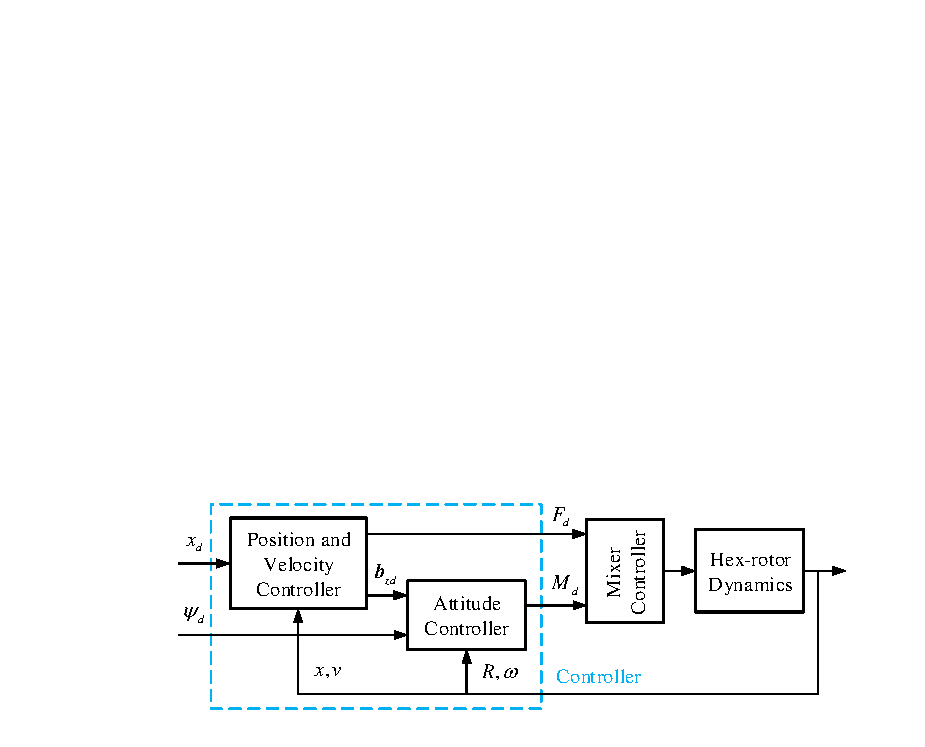
\includegraphics[width=2.95in]{illustrations/fig6.pdf}
    \caption{Control structure of hex-rotor}
    \label{f6}
\end{figure}

\section{Experimental Implementation}

\subsection{Overview of Experiment Setups}

The main experimental setups for wind disturbance rejection are shown in Fig. \ref{f7}.
The frame of the hex-rotor is DJI F550 using an open source control stack namely Pixhawk.
Table \ref{tab:1} shows some key features of our hex-rotor platform.
Wind disturbance is generated by an axial flow fan with $60cm$ diameters, and the maximum wind speed at outlet is up to $12m/s$ which is a level 6 wind and provides strong enough disturbance.
A 3-axis ultrasonic anemometer named WindMaster is used for wind velocity measuring.
The error of wind speed measurement is no more than $0.08m/s$ and wind direction is no more than $2^\circ$, and the sample rate is up to $32Hz$.
The effective range of wind speed measurement is $0\sim 65m/s$.
Moreover, since the experiment is carried out in indoor environment, we use a OptiTrack motion capture system, comprising with 8 cameras, to measure position and velocity of hex-rotor.
The error of position and velocity measurements is limited within $1cm$ and $0.2cm/s$ respectively with high sample rate at $50Hz$.
\begin{figure}[t]
    \centering
    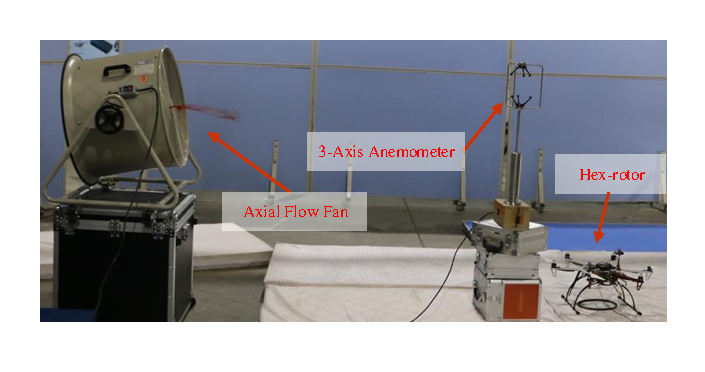
\includegraphics[width=2.95in]{illustrations/fig7.pdf}
    \caption{Experiental setups for wind disturbance rejection}
    \label{f7}
\end{figure}
\begin{table}[h]
    \centering
    \caption{Key Features of the Hex-rotor}
    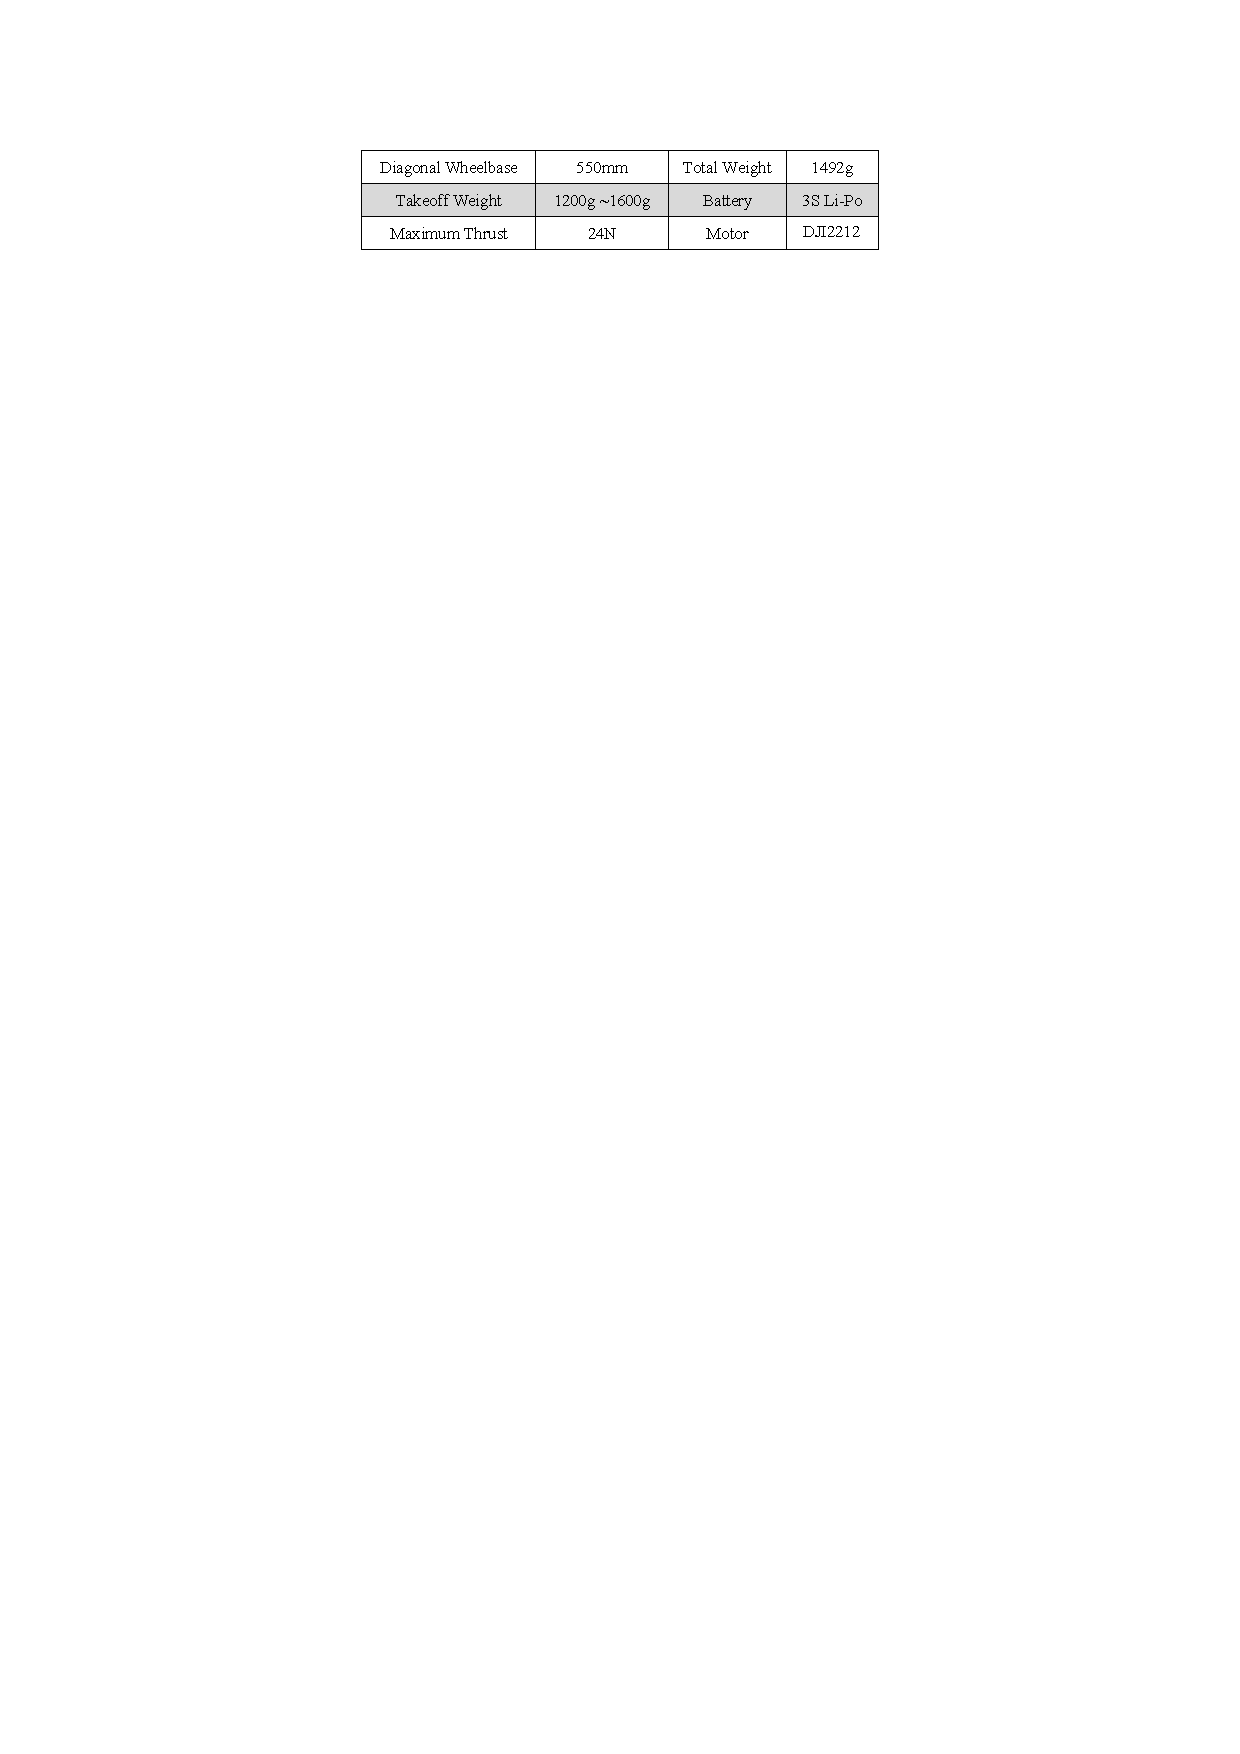
\includegraphics[width=3.2in]{illustrations/tab1.pdf}
    \label{tab:1}
\end{table}

\subsection{Online Acceleration Estimator}

As show in (\ref{e22}) and (\ref{e23}), the implementation of AF method needs real time measurement of linear and angular acceleration.
Acceleration information can be obtained by an onboard accelerometer integrated in Pixhawk.
However, the noise caused by rotation of six propellers is a tough problem.
Also, there is no angular accelerometer on hex-rotor since the cost is too high, and normally too heavy for UAV.
Thus, in our experiment, two online acceleration estimators based on \textsl{Kalman Filter} (KF) are designed.
One is for linear acceleration estimation using velocity information measured by motion capture system, and another is for angular acceleration estimation utilizing angular velocity measured by fusion of onboard gyroscope and accelerometer.
The model of KF for these two estimators can be generally described as
\begin{equation}
    \begin{bmatrix}
        x_{k+1} \\
        \dot{x}_{k+1}
    \end{bmatrix} = 
    \begin{bmatrix}
        1 & \Delta t_k \\
        0 & 1
    \end{bmatrix}
    \begin{bmatrix}
       x_k \\ \dot{x}_k
    \end{bmatrix}
    + \xi_k
    \label{e24}
\end{equation}
\begin{equation}
    z_k = x_k + \eta_k
    \label{e25}
\end{equation}
where $x_{k+1}$ and $x_k$ are true states and represents (angular) velocity at time $k+1$ and $k$, $\Delta t_k$ is the time interval,
and $\xi_k$ is the process noise which is assumed to be drawn form a zero mean multivariate normal distribution $\mathcal{N}$ with covariance $Q_k$, and $\xi_k\sim\mathcal{N}(0,Q_k)$.
$z_k$ is an observation at time $k$, and $\eta_k$ is the observation noise assumed to be zero mean Gaussian white noise with covariance $R_k$, and $\eta_k\sim\mathcal{N}(0,R_k)$.

The critical element for KF is the covariance of process and observation noise.
To determine $R_k$, we collect a set of data of (angular) velocity when the hex-rotor remains still, then the observation noise covariance can be decided by covariance analysis.
In our experiment, the noise covariance is chosen as Table \ref{tab:2}.
The online estimation results are demonstrated in Fig. \ref{f8}.
In each axis, there are three lines namely (angular) velocity, differential of (angular) velocity and KF estimation of (angular) acceleration.
As can be seen, differential and KF results always keep the same variation trend, but KF results turn out to be smoother and more suitable for online control.
\begin{figure}[t]
    \centering
    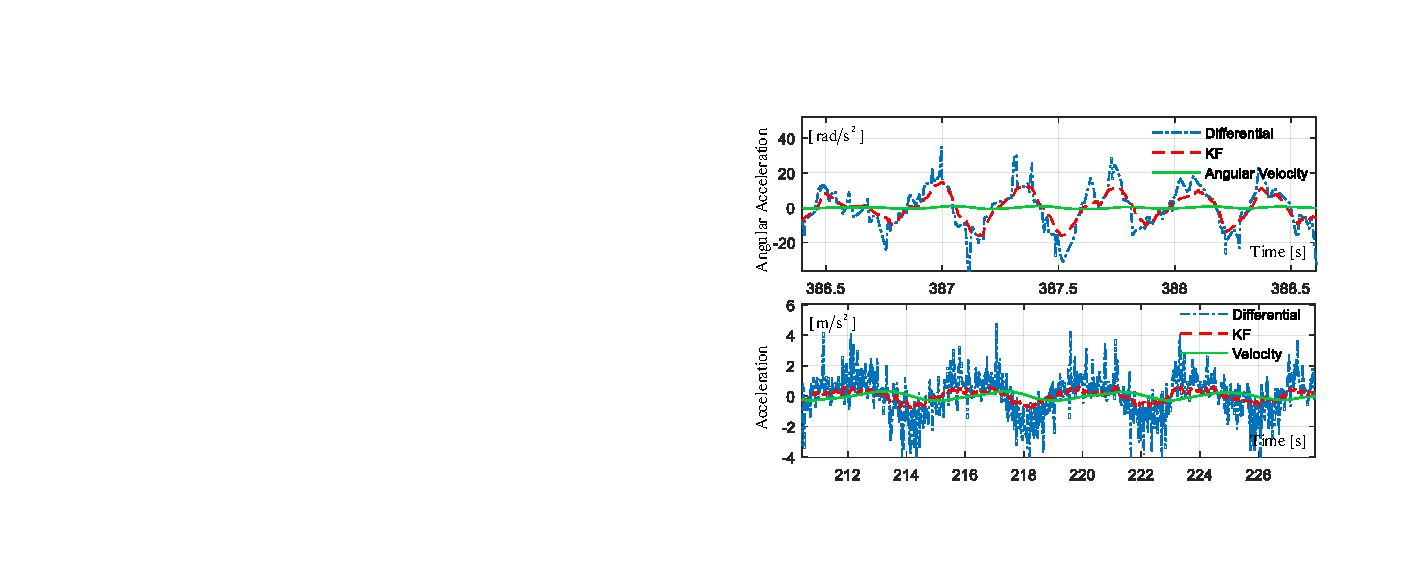
\includegraphics[width=2.95in]{illustrations/fig8.pdf}
    \caption{Estimation results of online KF}
    \label{f8}
\end{figure}
\begin{table}[t]
    \caption{Noise Covariance of KF}
    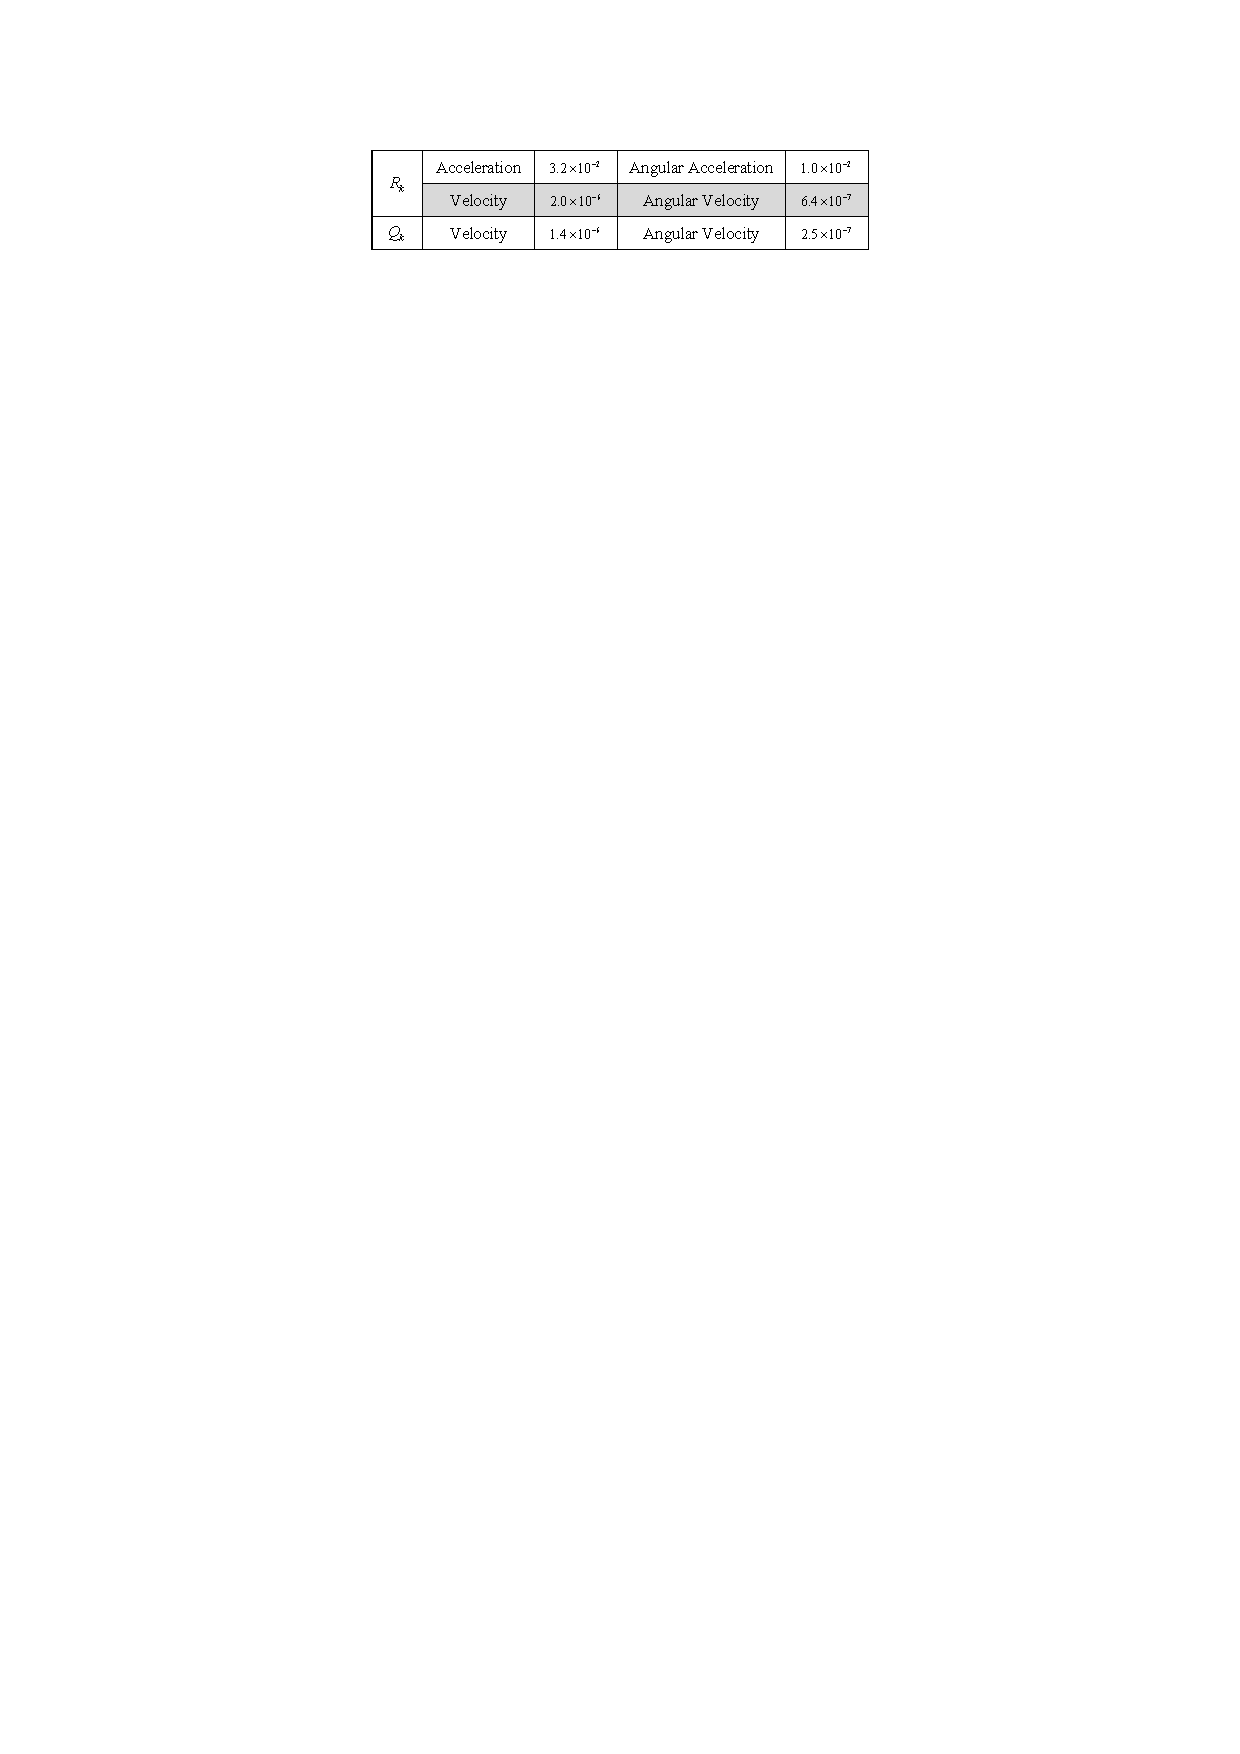
\includegraphics[width=3.2in]{illustrations/tab2.pdf}
    \centering
    \label{tab:2}
\end{table}

\subsection{An Novel Method for Parameters Identification}

From (\ref{e22}) and (\ref{e23}), we can conclude that AF is a model based method, and the implementation of AF needs to know the mass $m$, the moment of inertia $J$ and desired force $F_d$ and torque $M_d$ generated by controller.
$m$ is listed in Table \ref{tab:1}, and $J=diag(0.0145,0.0141,0.0266)$ is determined by bifilar pendulum method \cite{Soule1934}.

In fact, for most multi-rotor, we cannot control the force of the propellers directly since their motors are always controlled without speed closed-loop.
More specifically, the control input of motors is Pulse-Width Modulation (PWM) signal instead of rotating speed.
Moreover, in experiment, we found the same PWM signal may generate different rotating speed, mainly because the battery voltage continued decreasing over the whole flight test.
The control output $F_d$ generated by position and velocity PID controller shown in Fig. \ref{f6} is not a real force reference.
It’s a normalized value and its norm is limited from 0 to 1 corresponding to the minimum and maximum total thrust, namely $f_d$.
Thus, (\ref{e22}) cannot be used directly.
Fortunately, the relationship between $f_d$ and gravity can be determined by introducing an intermediate variable, that is battery voltage.
Based on this, a novel and simple method is proposed to solve these problems.

First, the hex-rotor needs to hover at a fixed point for a period to collect data of $f_d=[f_{dx},f_{dy},f_{dz}]$ and battery voltage $V$.
$f_{dx}$ and $f_{dy}$ can be considered as zero, and $f_{dz}$ is equivalent to gravity if the hovering accuracy is high enough.
Assume the relation between $f_{dy}$ and $V$ satisfy
\begin{equation}
    mg \Leftrightarrow f_{dz}=f(V)
    \label{e26}
\end{equation}
then
\begin{equation}
    m\ddot{x} \Leftrightarrow f(V)\frac{\ddot{x}}{g}
    \label{e27}
\end{equation}
Thus, conbining (\ref{e22}), we can obtain
\begin{equation}
    v_{Sf}(t) = a \int dt \left(
         f_d - f(V)(\bm{e}_3+\frac{\ddot{x}}{g})
        \right)
    \label{e28}
\end{equation}
where $v_{Sf}$ is the an scaled variable of $v_{f}$ in (\ref{e22}).
The relation between $f_{dz}$ and $V$ under hovering condition is fitted by a linear function.
The fitting result is illustrated in Fig. \ref{f9}.
The data we choose for fitting are from $150s$ to $330s$ where the hex-rotor is considered as hovering status, and the fitting function is
\begin{equation}
    f(V) = -0.0587V + 1.2435
    \label{e29}
\end{equation}
\begin{figure}[t]
    \centering
    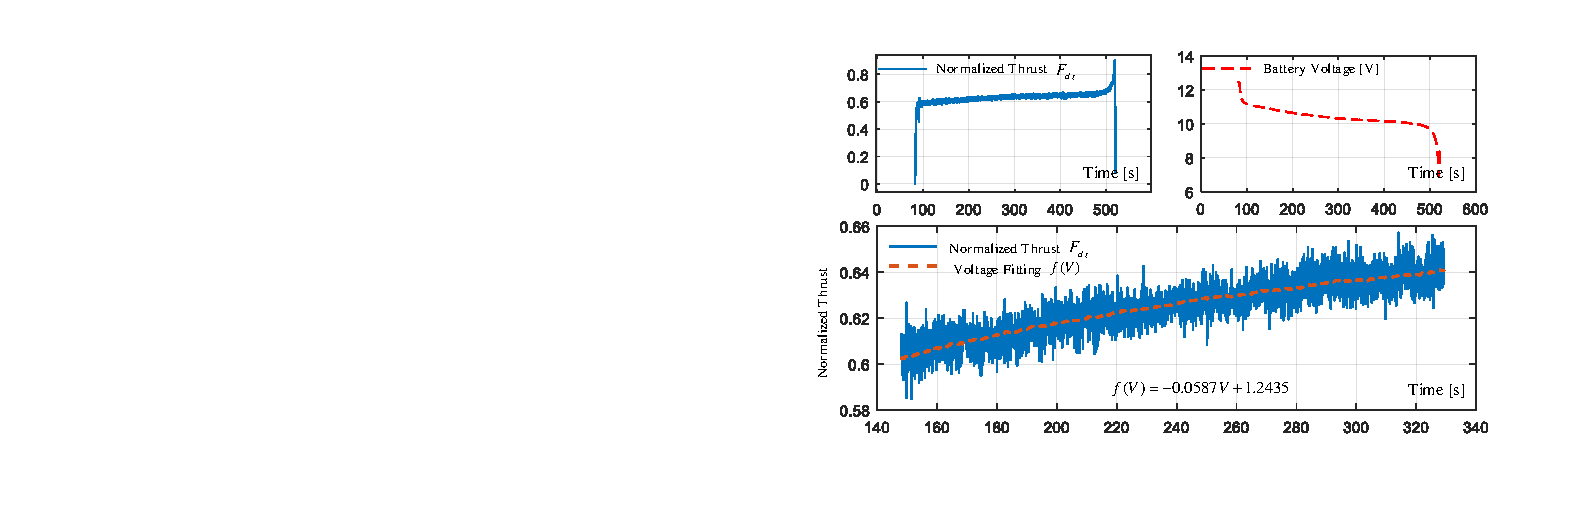
\includegraphics[width=2.95in]{illustrations/fig9.pdf}
    \caption{Fitting result between voltage and normalized thrust}
    \label{f9}
\end{figure}

The hovering test results with AF method are shown in Fig. \ref{f10}.
In the left two axes, $f(V) = 0.61$ is chosen as a constant without considering the relation with battery voltage, while in the right two axes, (\ref{e29}) is applied on AF enhanced controller.
As can be seen, the hovering accuracy increases largely in vertical and horizontal directions.
\begin{figure}[t]
    \centering
    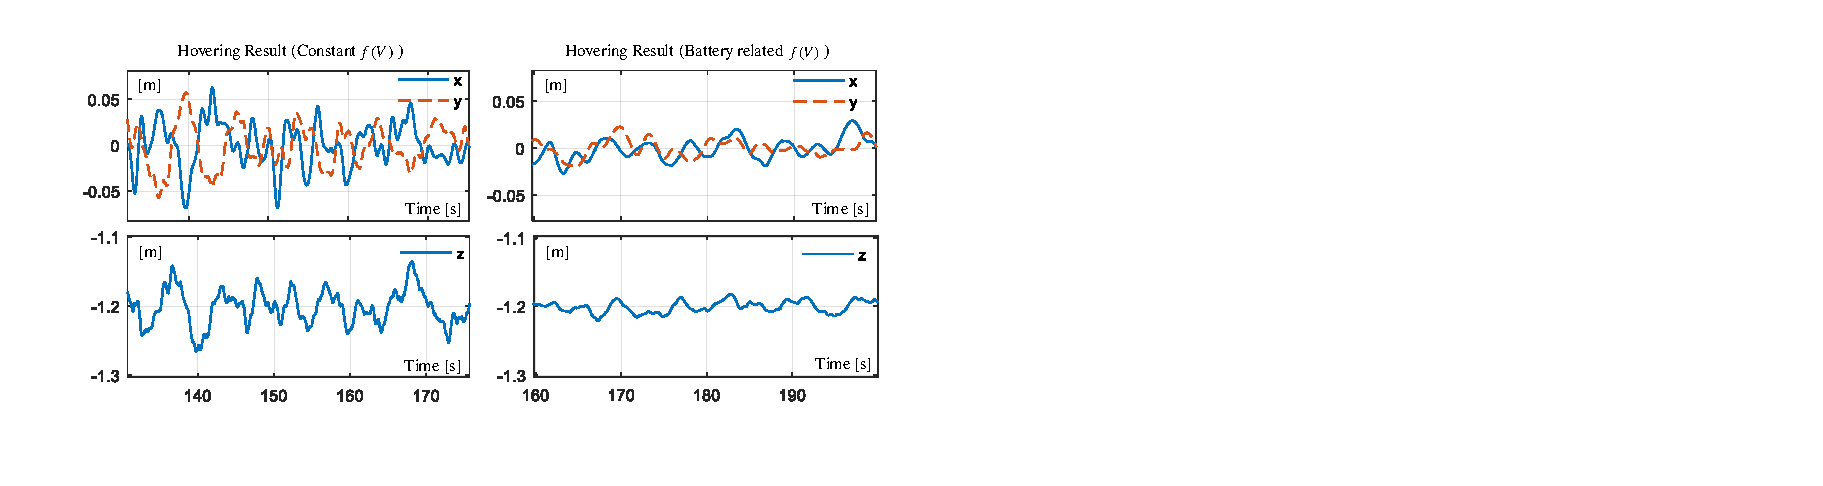
\includegraphics[width=2.95in]{illustrations/fig10.pdf}
    \caption{Hovering results at a fixed point with AF method}
    \label{f10}
\end{figure}

\section{Results Analysis}

In this section, two different strong winds, one is continuous wind and another is gusty wind, are taken into consideration, and the comparison of hovering performance between PID controller and AF enhanced PID controller under these two types of disturbances is presented.
Before this, to present that the disturbance generated by fan has practical significance we first give an analysis on various wind disturbance.

\subsection{Analyses on Wind Disturbances}

We collected about $50$ seconds of natural wind data in strong winds day.
As shown in Fig. \ref{f11}(top), the maximum speed of wind is up to $8m/s$, and the bottom shows the single-sided amplitude spectrum of the wind.
The constant component, where its frequency is $0Hz$, is nearly $6m/s$.
The amplitude of wind is lower than $0.4m/s$ at $0.3Hz$, and the bigger frequency is with lower amplitude.
Therefore, we can conclude that the frequency of natural wind is at low frequency level, which is important for AF enhanced controller design as discussed in Section II.
\begin{figure}[t]
    \centering
    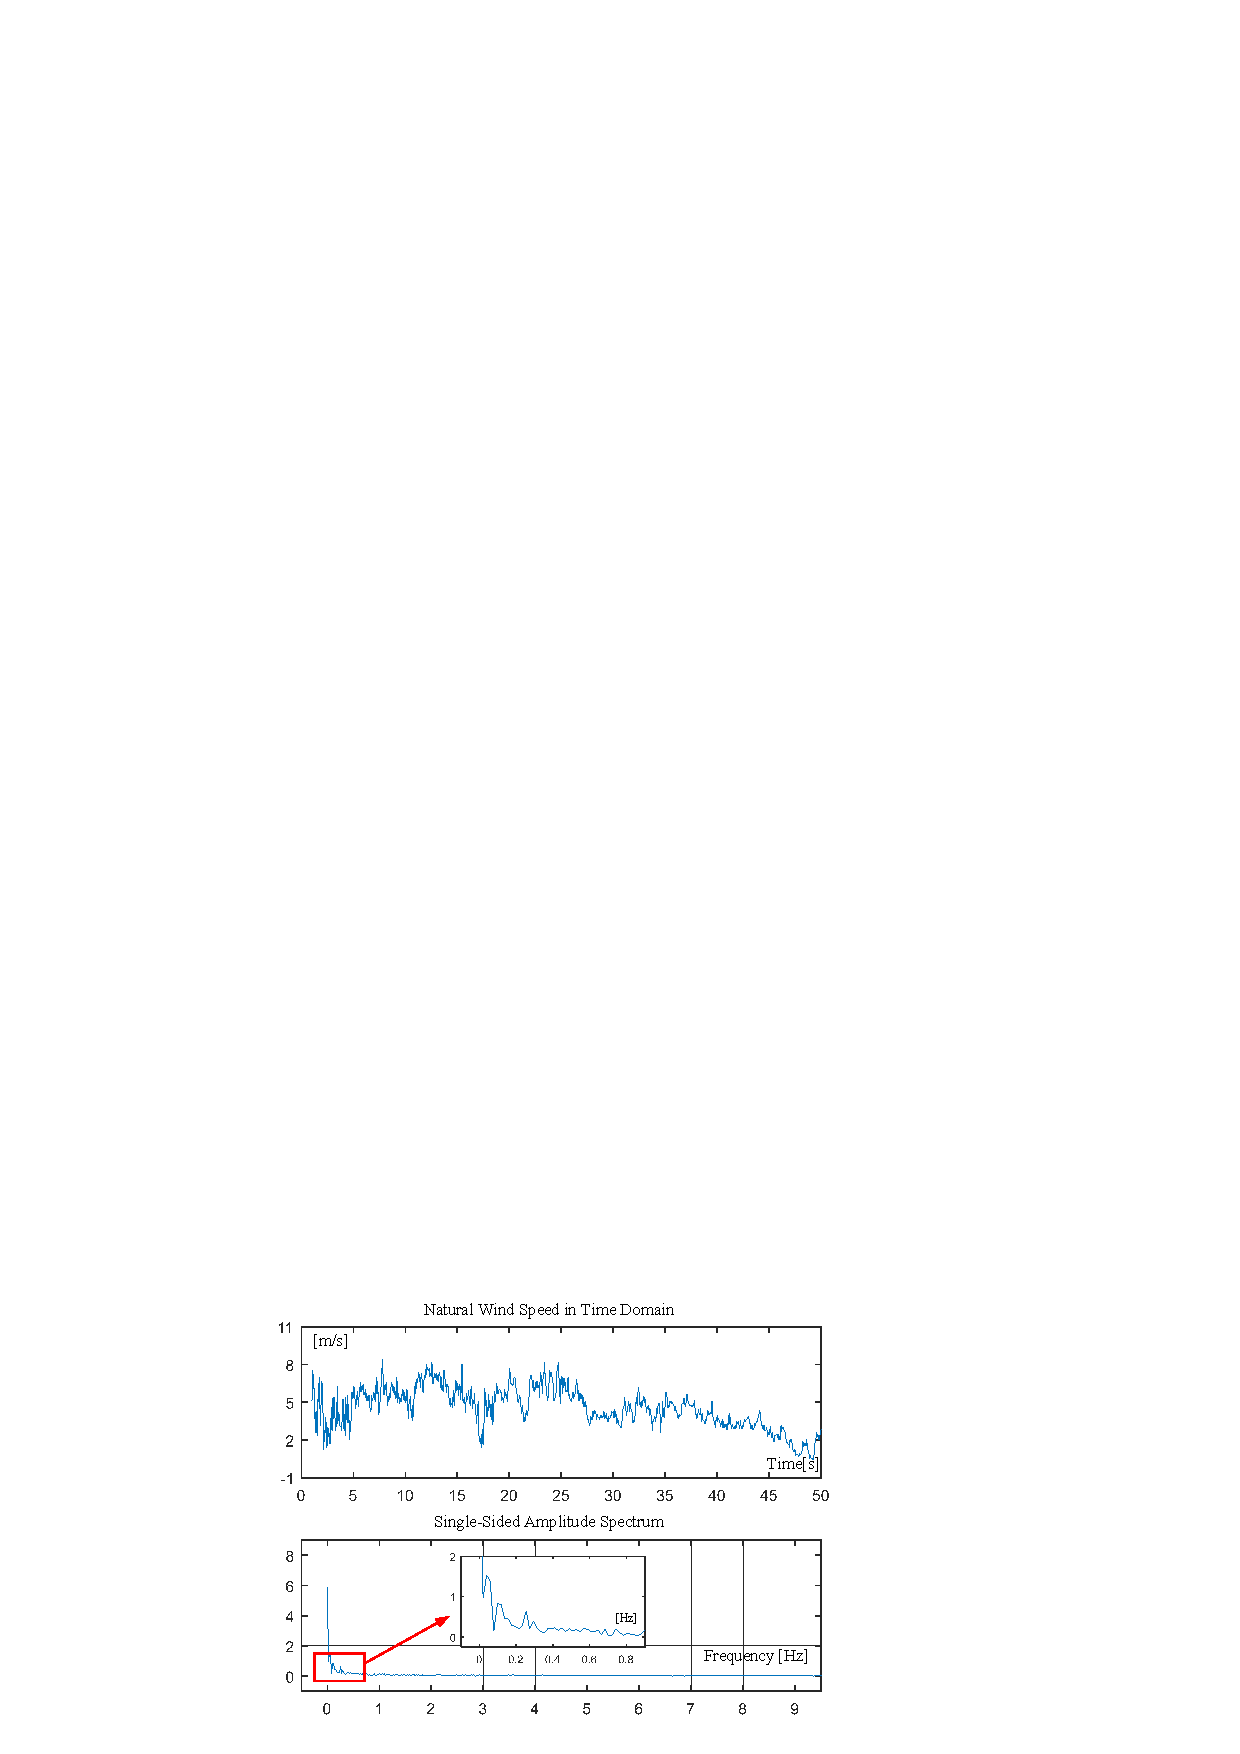
\includegraphics[width=2.95in]{illustrations/fig11.pdf}
    \caption{Hovering results at a fixed point with AF method}
    \label{f11}
\end{figure}

Two different strong winds, continuous and gusty wind, are collected and analyzed before the experiment as shown in Fig. \ref{f12} and Fig. \ref{f13} respectively, and the distance from the fan to desired hovering point are $1.8m$ and $2.2m$ respectively.
Continuous wind is generated by keeping the fan working all the time, while for gusty wind, the fan is turned on and off at a period of $3s$.
As can be seen in Fig. \ref{f12}, continuous wind has small fluctuates around a constant component about $7.8m/s$, and there is no large value at other frequencies.
While gusty wind, as shown in Fig. \ref{e13}, has smaller constant component about $6m/s$ since the further distance.
A more important feature is that the speed of gusty wind in time domain are more like a sine function, and its frequency, obviously shown in the spectrum result, is $0.31Hz$, where the amplitude is around $0.95m/s$.
Moreover, whether in continuous or gusty wind, there is a small component in Z-direction about $2m/s$ since the central axis of the fan is inclined about $7$ degrees.
From these analyses, we can conclude the wind generated by the fan is a well simulation of natural strong wind, which indicates our work has great practical significance.
\begin{figure}[t]
    \centering
    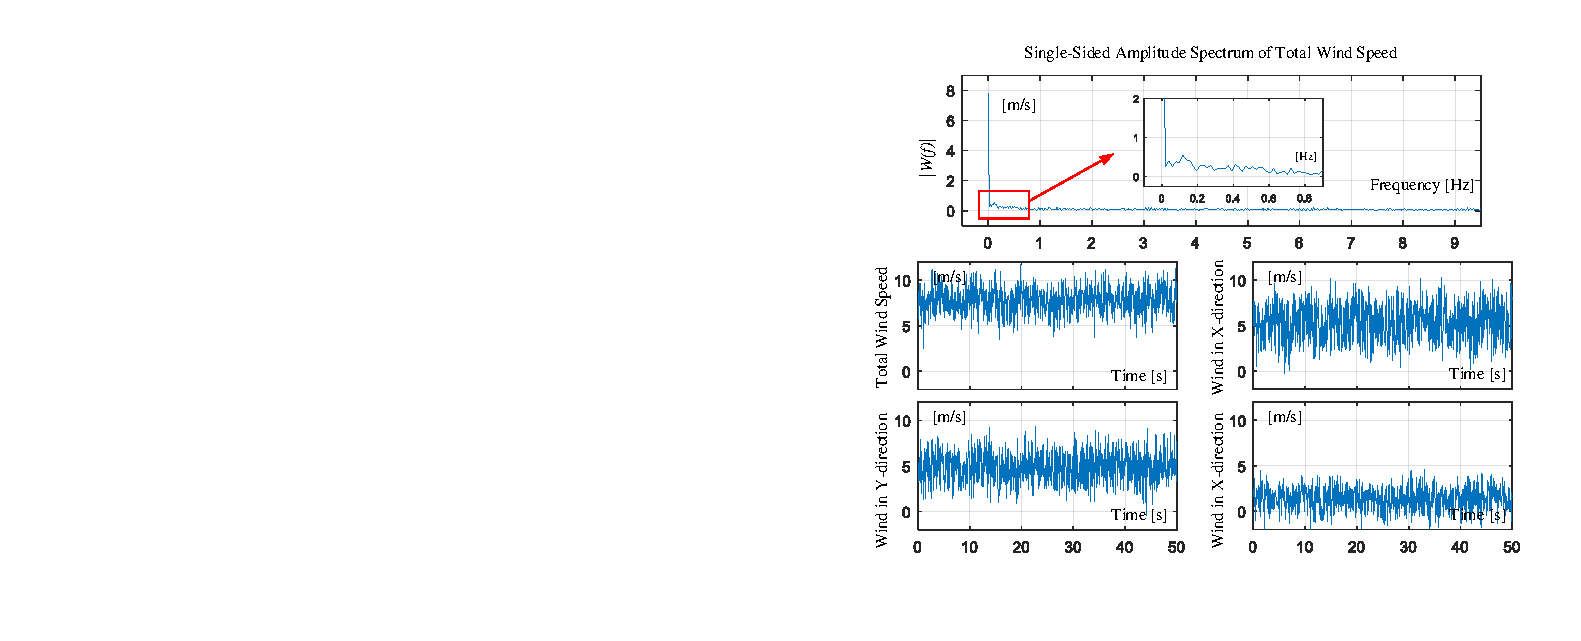
\includegraphics[width=2.95in]{illustrations/fig12.pdf}
    \caption{Continuous wind disturbance in time and frequency domain}
    \label{f12}
\end{figure}
\begin{figure}[t]
    \centering
    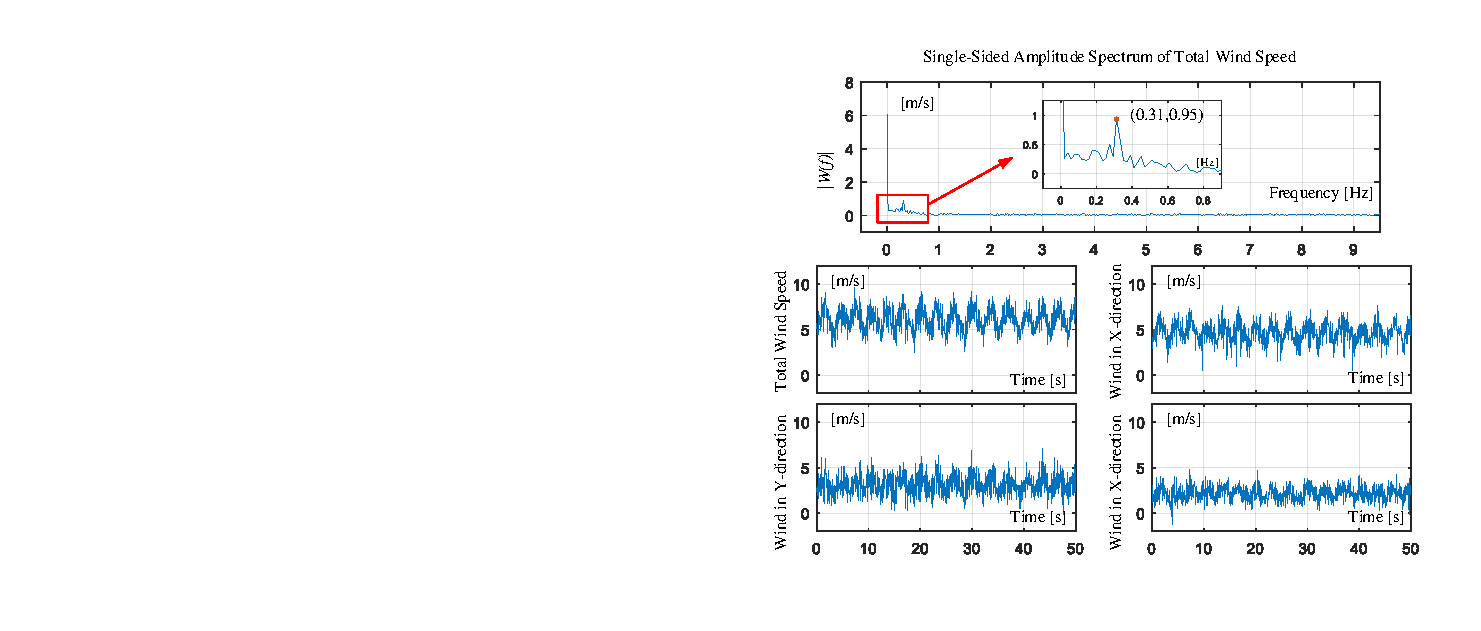
\includegraphics[width=2.95in]{illustrations/fig13.pdf}
    \caption{Gusty wind disturbance in time and frequency domain}
    \label{f13}
\end{figure}

\begin{figure}[t]
    \centering
    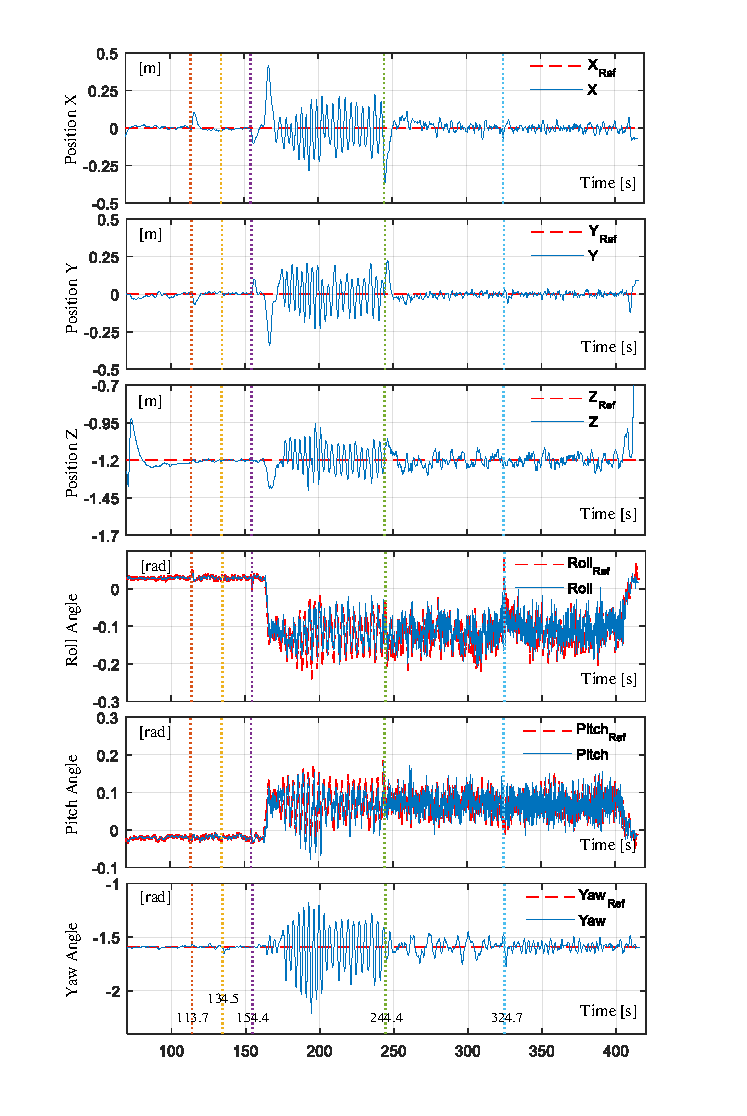
\includegraphics[width=2.95in]{illustrations/fig14.pdf}
    \caption{ Experimental results of disturbance rejection for continuous wind}
    \label{f14}
\end{figure}

\subsection{Disturbance Rejection for Continuous Wind}

The disturbance rejection for continuous wind can be divided into two parts: the hovering test under no wind condition and strong continuous wind condition, and each part contains a PID controller test and two AF enhanced controller test, namely linear AF enhanced (L-AF) controller (Linear AF and PID) and linear and angular AF enhanced (LA-AF) controller (Linear and angular AF and PID).
The flight test results are shown in Fig. \ref{f14}, and the moments of controller switching are label in the bottom.
Before $113.7s$, the hex-rotor takes off and hovers at a fix point $(0,0,-1.2)^T$ with PID controller.
Then, from $113.7s$ to $134.5s$, the controller is switched to LA-F controller, and from $134.5s$ to $154.4s$, the LA-AF enhanced controller is used.
Then, at $154.4s$ the controller is switched back to PID and the fan is turned on.
From $244.4s$ to $324.7s$, the LA-F controller is used, and at $324.7s$, the controller is switch to LA-AF controller again.
Finally, the hex-rotor starts landing at $400s$.

The results show a good performance of AF enhanced method.
First, under no wind condition, AF enhanced controller performs as well as PID controller.
Then, after the fan turned on, the L-AF controller is more stable and a higher accuracy of position and attitude (Yaw angle) has been achieved compared to PID.
Moreover, when LA-AF controller is applied at $324.7s$, the accuracy of yaw angle is further promoted.
The root mean square errors (RMSEs) of position and yaw are listed in Table \ref{tab:3}.
Compared with PID controller, the accuracy of LA-AF controller is $4.8$ times higher on position and $5.2$ times higher on yaw angle.
\begin{table}[t]
    \caption{RMSEs under Continuous Wind}
    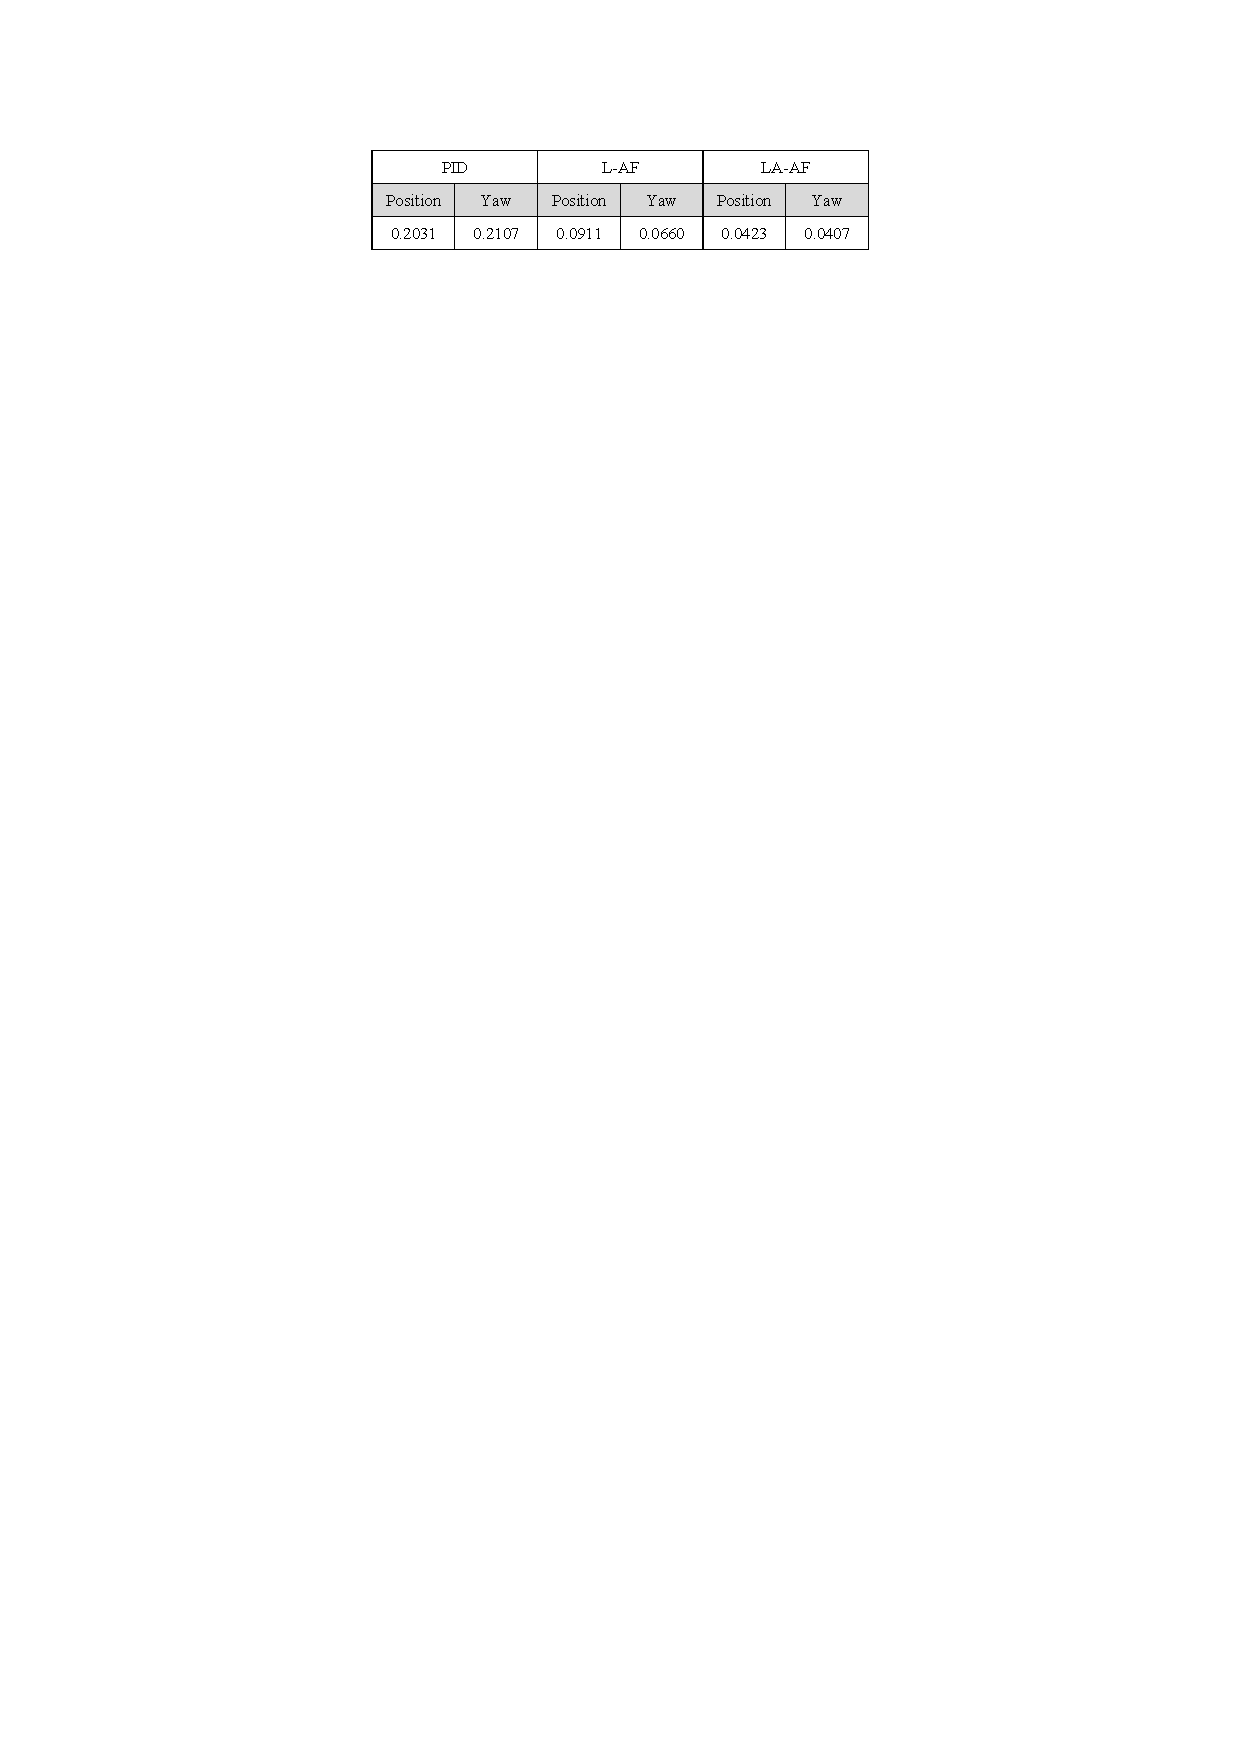
\includegraphics[width=3.2in]{illustrations/tab3.pdf}
    \centering
    \label{tab:3}
\end{table}

However, there are some points that need to be clear here.
Firstly, there is a little hump of the data shown in Fig. \ref{f14} right after controller switched, which is caused by the interaction between (\ref{e22}) or (\ref{e23}) and integral part of PID.
Secondly, the attitude (roll and pitch) changes more acutely when applied AF enhanced method, so that it can suppress disturbance faster and better.
Thirdly, the error of position has periodicity is because the wind is too strong that hex-rotor is blowed out of the wind field.
Finally, the improvement of position accuracy in Z-axis is lower than it in X-axis and Y-axis since vertical disturbance effects thrust of propellers directly.

\subsection{Disturbance Rejection for Gusty Wind}

The results of disturbance rejection for gusty wind are shown in Fig. \ref{f15}.
This time, the hex-rotor stay in the wind all the time rather blowed out of wind field.
When the hex-rotor hovers steady, the fan is turned on at $142.5s$, and LA-AF controller is applied at $232s$.
The RMSEs of position and yaw under gusty wind are shown in Table \ref{tab:4}.
Compared with PID controller, the accuracy of LA-AF controller is $2.6$ times higher on position and $3.3$ times higher on yaw angle.
\begin{figure}[t]
    \centering
    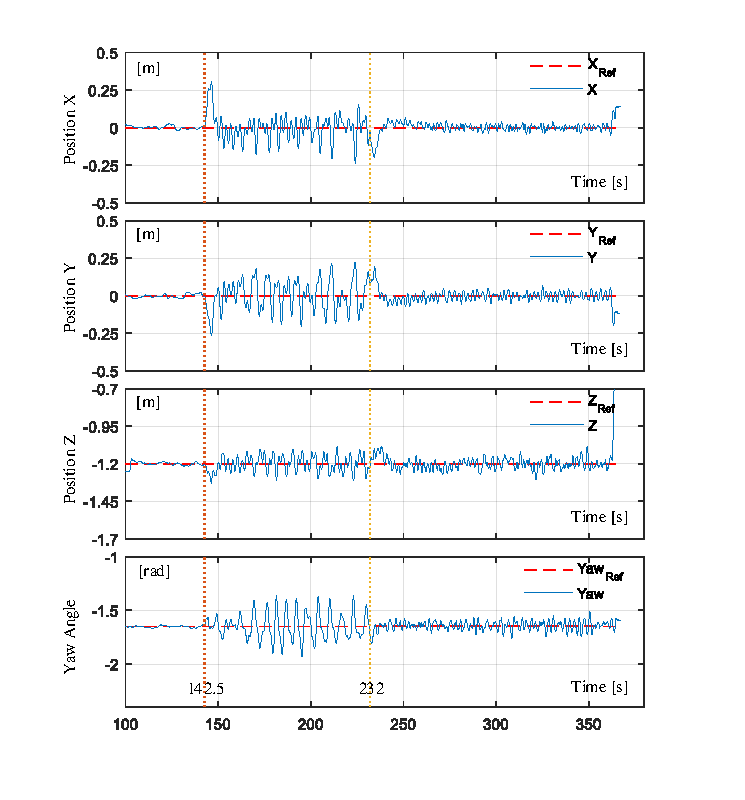
\includegraphics[width=2.95in]{illustrations/fig15.pdf}
    \caption{ Experimental results of disturbance rejection for gusty wind}
    \label{f15}
\end{figure}
\begin{table}[t]
    \caption{RMSEs under Gusty Wind}
    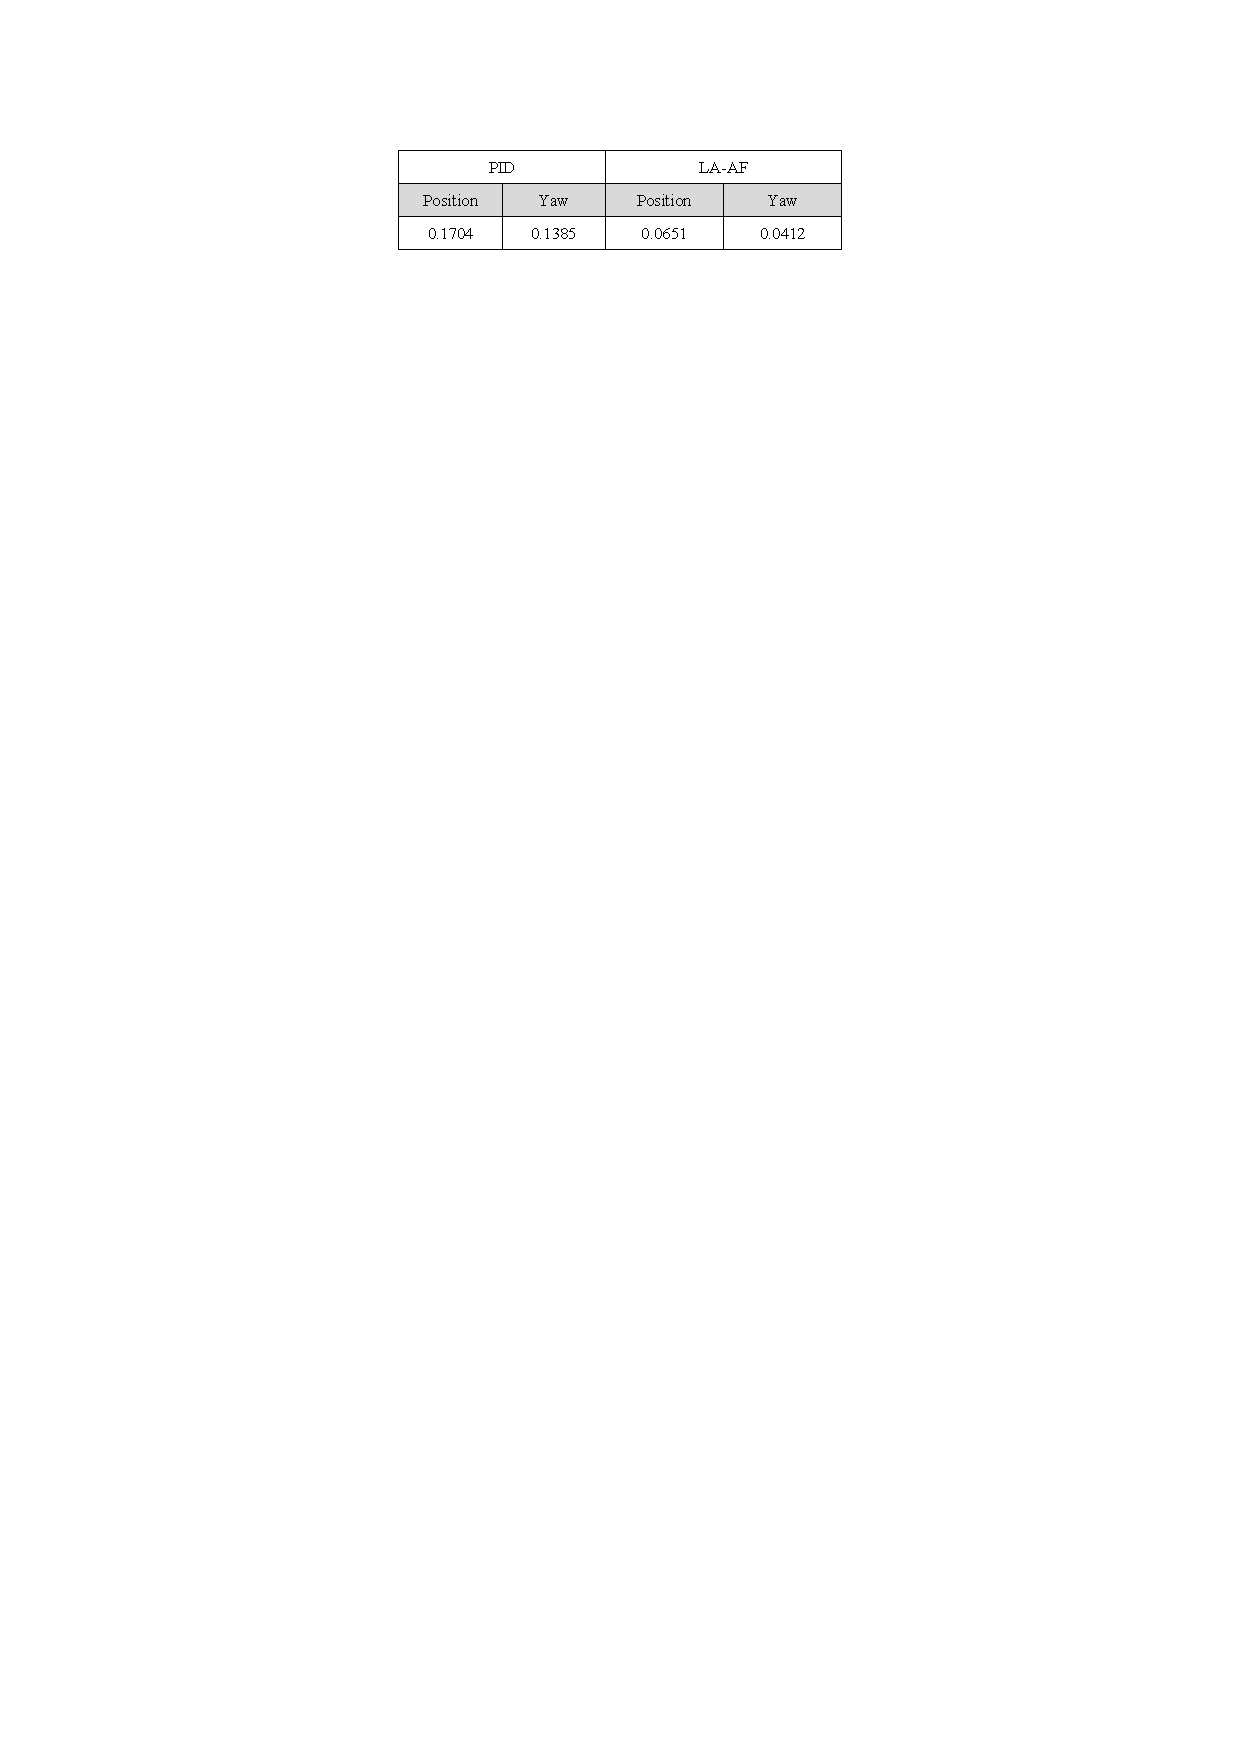
\includegraphics[width=2.95in]{illustrations/tab4.pdf}
    \centering
    \label{tab:4}
\end{table}

\section{Conclusion}

This paper presents an acceleration feedback method for enhancing the controller of UAV to reject wind disturbance.
A modified method of traditional high gain acceleration feedback is used to eliminate the algebraic loop and make it easier to be implemented.
To apply this method on a model free controller such as PID, a novel and simple method for parameters identification is proposed, and the results of the experiment have verified its effectiveness.
In addition, the analyses of different types of winds demonstrate the wind disturbance generated by fan is very similar with natural strong wind, which turns out that our research is authentic and practical.
At last, the experimental results for disturbance rejection under continuous and gusty winds demonstrate the effectiveness and robustness of our acceleration feedback method.
Thus, it is promising to apply this method on future disturbance rejection applications.

\addtolength{\textheight}{-12cm}   % This command serves to balance the column lengths
                                  % on the last page of the document manually. It shortens
                                  % the textheight of the last page by a suitable amount.
                                  % This command does not take effect until the next page
                                  % so it should come on the page before the last. Make
                                  % sure that you do not shorten the textheight too much.

% \begin{thebibliography}{99}

% \end{thebibliography}
\bibliographystyle{IEEEtran}
\bibliography{refs}



\end{document}
